\documentclass[../main]{subfiles}
\begin{document}

\chapter{抽样定理}%
\label{cha:sample}

% \section{实验目的}%
% \label{sec:\arabic{chapter}aim}
%
% \begin{itemize}
%   \item 了解抽样定理在通信系统中的重要性。
%   \item 掌握自然抽样及平顶抽样的实现方法。
%   \item 理解低通采样定理的原理。
%   \item 理解实际的抽样系统。
%   \item 理解低通滤波器的幅频特性对抽样信号恢复的影响。
%   \item 理解低通滤波器的相频特性对抽样信号恢复的影响。
%   \item 理解带通采样定理的原理。
% \end{itemize}
%
% \section{实验器材}%
% \label{sec:\arabic{chapter}equipment}
%
% \begin{table}[htbp]
%   \centering
%   \caption{实验器材}%
%   \label{tab:\arabic{chapter}equipment}
%   \csvautobooktabular[respect percent]{tab/\arabic{chapter}equipment.csv}
% \end{table}
%
\section{实验原理}%
\label{sec:\arabic{chapter}principle}

\begin{figure}[htbp]
  \centering
  \includegraphics[
    width = 0.8\linewidth,
  ]{\arabic{chapter}dia}
  \caption{实验原理框图}%
  \label{fig:\arabic{chapter}dia}
\end{figure}

抽样信号由抽样电路产生。将输入的被抽样信号与抽样脉冲相乘就可以得到自然抽样信
号,自然抽样的信号经过保持电路得到平顶抽样信号。平顶抽样和自然抽样信号是通过
开关 S1 切换输出的。

抽样信号的恢复是将抽样信号经过低通滤波器,即可得到恢复的信号。这里滤波器可以
选用抗混叠滤波器(8 阶 3.4kHz 的巴特沃斯低通滤波器)或 FPGA 数字滤波器(有
FIR、 IIR 两种)。反 sinc 滤波器不是用来恢复抽样信号的,而是用来应对孔径失真
现象。要注意,这里的数字滤波器是借用的信源编译码部分的端口。在做本实验时与信
源编译码的内容没有联系。

\section{实验步骤}%
\label{sec:\arabic{chapter}procedure}

\subsection{抽样信号观测及抽样定理验证}%
\label{sub:sample}

% 通过不同频率的抽样时钟,从时域和频域两方面观测自然抽样和平顶抽样的输出波形,
% 以及信号恢复的混叠情况,从而了解不同抽样方式的输出差异和联系,验证抽样定理。

% \begin{table}[htbp]
%   \centering
%   \caption{连线}%
%   \label{tab:\arabic{chapter}\arabic{subsection}}
%   \small
%   \csvautobooktabular[respect percent]{tab/\arabic{chapter}\arabic{subsection}.csv}
% \end{table}

% \begin{enumerate}
%   \item 关电,按表~\ref{tab:\arabic{chapter}\arabic{subsection}}所示进行连线
%     。
%   \item 开电,设置主控菜单,选择【主菜单】→【通信原理】→【抽样定理】。调节主
%     控模块的 W1 使 A-OUT 输出峰峰值为 3V。
%   \item 此时实验系统初始状态为:被抽样信号 MUSIC 为幅度 4V、频率 3K+1K 正弦合
%     成波。抽样脉冲 A-OUT 为幅度 3V、频率 9kHz、占空比 20\%的方波。
%   \item 实验操作及波形观测。
  \begin{enumerate}
    \item 观测并记录自然抽样前后的信号波形:设置开关 S1 3\# 为“自然抽样”档位
      ,用示波器分别观测 MUSIC (主控\&信号源)和抽样输出 3\#
      图~\ref{fig:sample/nature}。
    \item 观测并记录平顶抽样前后的信号波形:设置开关 S1 3\# 为“平顶抽样”档位
      ,用示波器分别观测 MUSIC (主控\&信号源)和抽样输出 3\#
      图~\ref{fig:sample/flat}。
    \item 观测并对比抽样恢复后信号与被抽样信号的波形:设置开关 S1 3\# 为“自然
      抽样”档位,用示波器观测 MUSIC (主控\&信号源)和 LPF-OUT
      3\# 图~\ref{fig:analog},以 100Hz 的步进减小 A-OUT (主控\&信号源)的频率
      。

      \begin{Exercise}[title = 思考]
        比较观测并思考在抽样脉冲频率多小的情况下恢复信号有失真。
      \end{Exercise}

      \begin{Answer}
        理论上只有当抽样脉冲频率小于 8kHz 时才会失真,但实际上由于低通滤波器
        并非理想低通,实际阈值将大于 8kHz。当以 100Hz 的步进减小抽样频率时,
        如图~\ref{fig:analog},可以发现在刚好 8kHz 时时域有一定失真,从而证明
        了该滤波器不够理想。而在频域,从图~\ref{fig:freqsample/lp}和
        图~\ref{fig:freqsample/unsample}的对比亦可发现该滤波器没完全滤去除
        1kHz 和 3kHz 以外不需要的频谱。
      \end{Answer}

    \item 用频谱的角度验证抽样定理(选做):用示波器频谱功能观测并记录被抽样
      信号 MUSIC 图~\ref{fig:freqsample/unsample} 和抽样输出频谱
      图~\ref{fig:freqsample/sample}。以 100Hz 的步进减小抽样脉冲的频率,观测
      抽样输出图~\ref{fig:freqsample/sample}以及恢复信号的频谱
      图~\ref{fig:freqsample/lp}。\footnote{观察
        图~\ref{fig:freqsample/unsample}和图~\ref{fig:freqsample/sample}可发
      现出现了周期延拓}(注意:示波器需要用 250kSa/s 采样率(
      即每秒采样点为 250k),FFT 缩放调节为$\times 10$)。
  \end{enumerate}
% \end{enumerate}

\begin{figure}[htbp]
  \centering
  \begin{subfigure}[htbp]{0.45\linewidth}
    \centering
    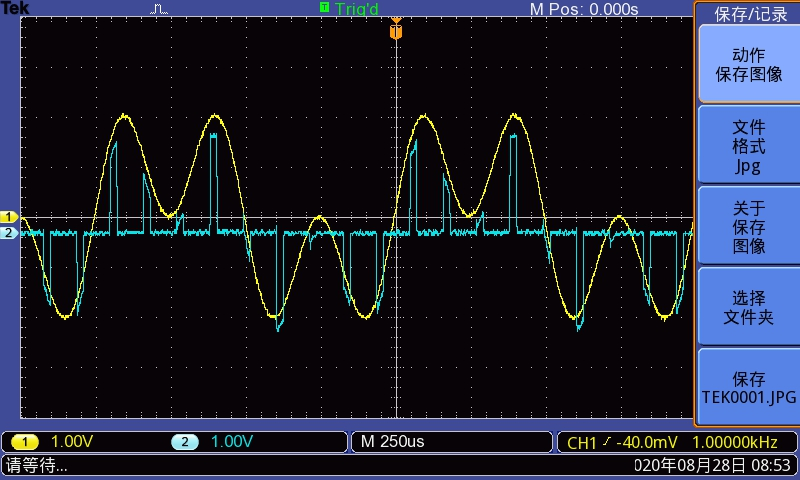
\includegraphics[
      width = \linewidth,
    ]{sample/nature}
    \caption{自然抽样}%
    \label{fig:sample/nature}
  \end{subfigure}
  \quad
  \begin{subfigure}[htbp]{0.45\linewidth}
    \centering
    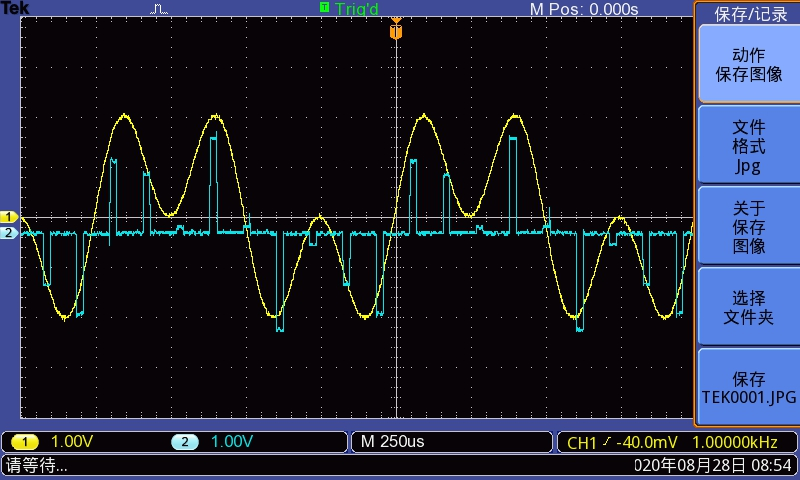
\includegraphics[
      width = \linewidth,
    ]{sample/flat}
    \caption{平顶抽样}%
    \label{fig:sample/flat}
  \end{subfigure}
  \caption{抽样}%
  \label{fig:sample}
\end{figure}

\begin{figure}[htbp]
  \centering
  \begin{subfigure}[htbp]{0.45\linewidth}
    \centering
    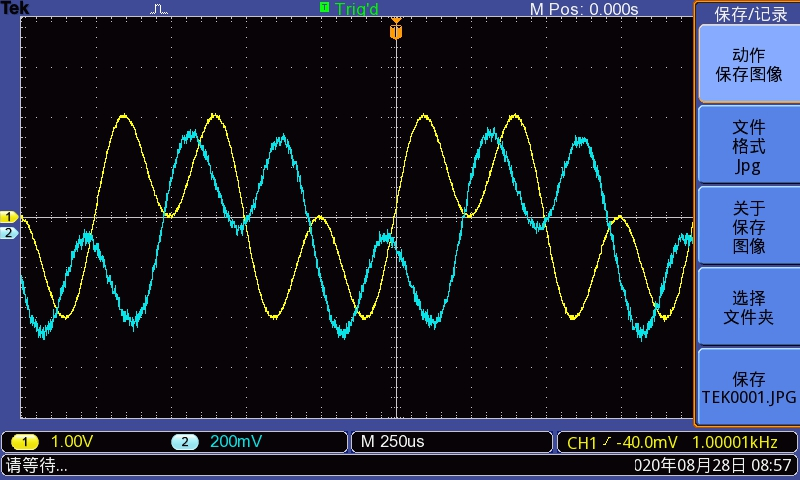
\includegraphics[
      width = \linewidth,
    ]{analog/recover}
    \caption{还原}%
    \label{fig:analog/recover}
  \end{subfigure}
  \quad
  \begin{subfigure}[htbp]{0.45\linewidth}
    \centering
    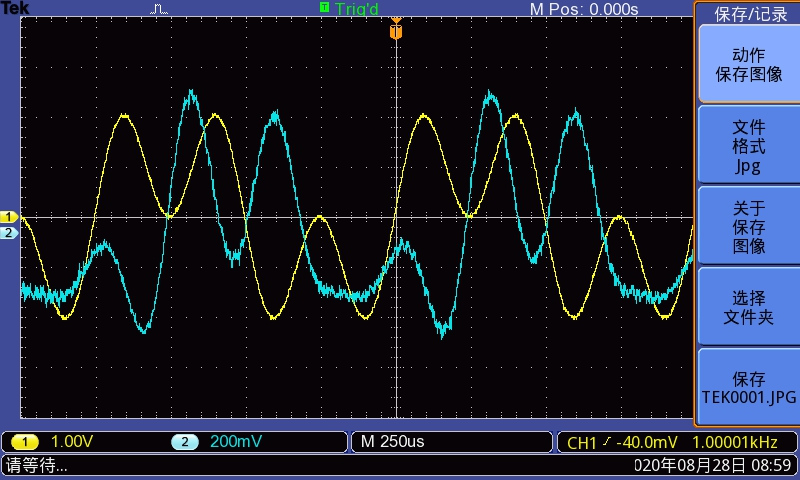
\includegraphics[
      width = \linewidth,
    ]{analog/distortion}
    \caption{失真}%
    \label{fig:analog/distortion}
  \end{subfigure}
  \caption{模拟低通滤波}%
  \label{fig:analog}
\end{figure}

\begin{figure}[htbp]
  \centering
  \begin{subfigure}[htbp]{0.45\linewidth}
    \centering
    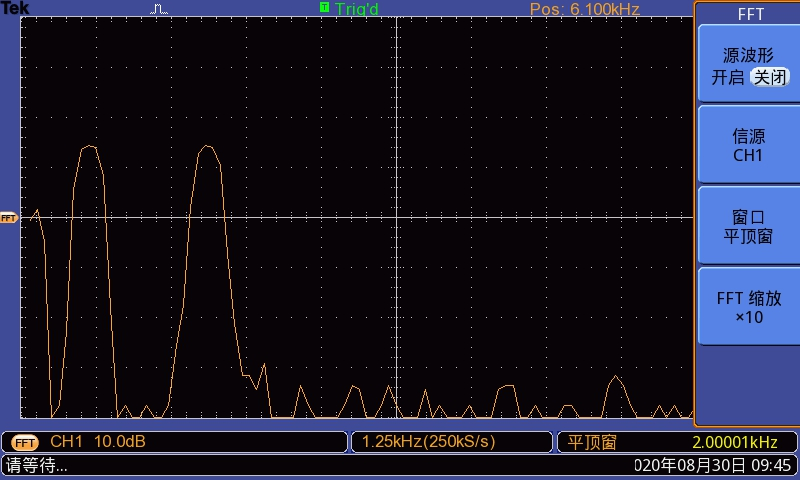
\includegraphics[
      width = \linewidth,
    ]{freqsample/unsample}
    \caption{被抽样信号}%
    \label{fig:freqsample/unsample}
  \end{subfigure}
  \quad
  \begin{subfigure}[htbp]{0.45\linewidth}
    \centering
    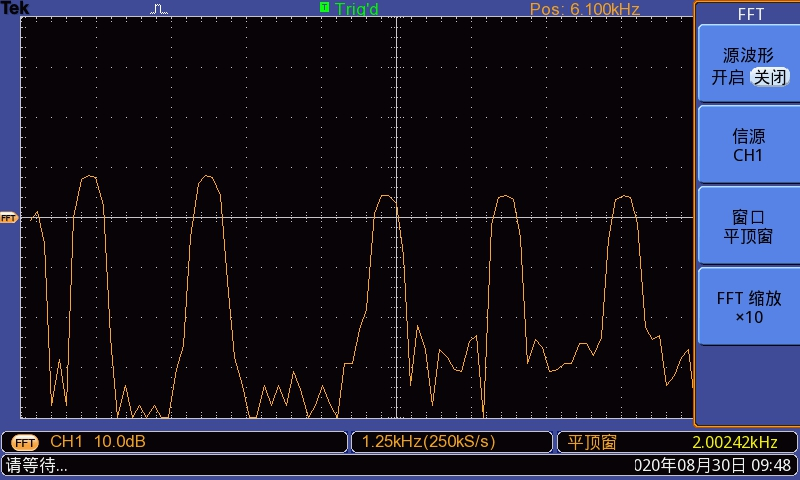
\includegraphics[
      width = \linewidth,
    ]{freqsample/sample}
    \caption{抽样输出}%
    \label{fig:freqsample/sample}
  \end{subfigure}

  \begin{subfigure}[htbp]{0.45\linewidth}
    \centering
    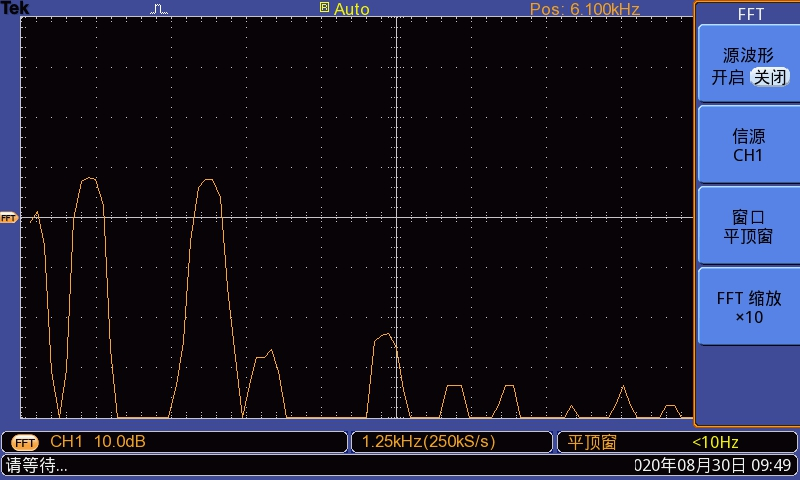
\includegraphics[
      width = \linewidth,
    ]{freqsample/lp}
    \caption{模拟低通滤波器还原}%
    \label{fig:freqsample/lp}
  \end{subfigure}
  \caption{频谱抽样}%
  \label{fig:freqsample}
\end{figure}

% 注:通过观测频谱可以看到当抽样脉冲小于 2 倍被抽样信号频率时,信号会产生混叠。

\subsection{滤波器幅频特性对抽样信号恢复的影响}%
\label{sub:freq}

% 该项目是通过改变不同抽样时钟频率,分别观测和绘制抗混叠低通滤波和 fir 数字滤波
% 的幅频特性曲线,并比较抽样信号经这两种滤波器后的恢复效果,从而了解和探讨不同
% 滤波器幅频特性对抽样信号恢复的影响。

\subsubsection{测试抗混叠低通滤波器的幅频特性曲线}%
\label{ssub:lp}

% \begin{table}[htbp]
%   \centering
%   \caption{连线}%
%   \label{tab:\arabic{chapter}\arabic{subsection}lp}
%   \csvautobooktabular[respect percent]{tab/\arabic{chapter}\arabic{subsection}lp.csv}
% \end{table}

% \begin{enumerate}
%   \item 关电,按表~\ref{tab:\arabic{chapter}\arabic{subsection}lp}所示进行连
%     线。
%   \item 开电,设置主控模块,选择【信号源】→【输出波形】和【输出频率】,通过调
%     节相应旋钮,使 A-OUT (主控\& 信号源) 输出频率 5kHz、峰峰值为 3V 的正弦波
%     。
%   \item 此时实验系统初始状态为:抗混叠低通滤波器的输入信号为频率 5kHz、幅度
%     3V 的正弦波。
%   \item 实验操作及波形观测。

  \begin{enumerate}
    \item 用示波器观测 LPF-OUT 3\# 。以 100Hz 步进减小
      A-OUT LPF-OUT 3\# 的频谱。记入表\footnote{篇幅要求,删表留图,后面同此
      。}。
    \item 由上述表,画出模拟低通滤波器幅频特性曲线图~\ref{fig:freq}。
  \end{enumerate}
% \end{enumerate}

% \begin{table}[htbp]
%   \centering
%   \caption{幅频特性}%
%   \label{tab:freq}
%   \begin{subtable}[htbp]{0.45\linewidth}
%     \centering
%     \caption{抗混叠低通滤波器}%
%     \label{tab:iir}
%     \tiny
%     \csvautobooktabular[respect percent]{tab/lp.csv}
%   \end{subtable}
%   \quad
%   \begin{subtable}[htbp]{0.45\linewidth}
%     \centering
%     \caption{数字滤波器}%
%     \label{tab:fir}
%     \tiny
%     \csvautobooktabular[respect percent]{tab/fir.csv}
%   \end{subtable}
% \end{table}

\begin{Exercise}[title = 思考]
  对于 3.4kHz 低通滤波器,为了更好的画出幅频特性曲线,我们可以如何调整信号源
  输入频率的步进值大小?
\end{Exercise}

\begin{Answer}
  应该在 3.4kHz 附近多取采样点以保证采样点依次连接而成的折线图与真实的函数曲
  线的均方误差更小。而离 3.4kHz 较远的地方可以少取采样点。因为幅频曲线只在通
  频带范围内变化剧烈。
\end{Answer}

\subsubsection{测试 fir 数字滤波器的幅频特性曲线}%
\label{ssub:fir}

% \begin{table}[htbp]
%   \centering
%   \caption{连线}%
%   \label{tab:\arabic{chapter}\arabic{subsection}fir}
%   \csvautobooktabular[respect percent]{tab/\arabic{chapter}\arabic{subsection}fir.csv}
% \end{table}

% \begin{enumerate}
%   \item 关电,按表~\ref{tab:\arabic{chapter}\arabic{subsection}fir}
%     所示进行连线。
%   \item 开电,设置主控菜单:选择【主菜单】→【通信原理】→【抽样定理】→【FIR 滤
%     波器】。调节【信号源】,使 A-OUT 输出频率 5kHz、峰峰值为 3V 的正弦波。
%   \item 此时实验系统初始状态为:fir 滤波器的输入信号为频率 5kHz、幅度 3V 的正弦波。
%   \item 实验操作及波形观测。

  \begin{enumerate}
    \item 用示波器观测译码输出 3\#,以 100Hz 的步进减小
      A-OUT (主控\& 信号源)的频率。观测并记录译码输出 3\#的频谱。记入表。
    \item 由上述表,画出 fir 低通滤波器幅频特性曲线图~\ref{fig:freq}。
  \end{enumerate}
% \end{enumerate}

\begin{Exercise}[title = 思考]
  对于 3kHz 低通滤波器,为了更好的画出幅频特性曲线,我们可以如何调整信号源输
  入频率的步进值大小?
\end{Exercise}

\begin{Answer}
  应该在 3kHz 附近多取采样点以保证采样点依次连接而成的折线图与真实的函数曲线
  的均方误差更小。而离 3kHz 较远的地方可以少取采样点。因为幅频曲线只在通
  频带范围内变化剧烈。
\end{Answer}

\begin{figure}[htbp]
  \centering
  \begin{subfigure}[htbp]{0.45\linewidth}
    \centering
    \includegraphics[
      width = \linewidth,
    ]{freq}
    \caption{幅频特性}%
    \label{fig:freq}
  \end{subfigure}
  \quad
  \begin{subfigure}[htbp]{0.45\linewidth}
    \centering
    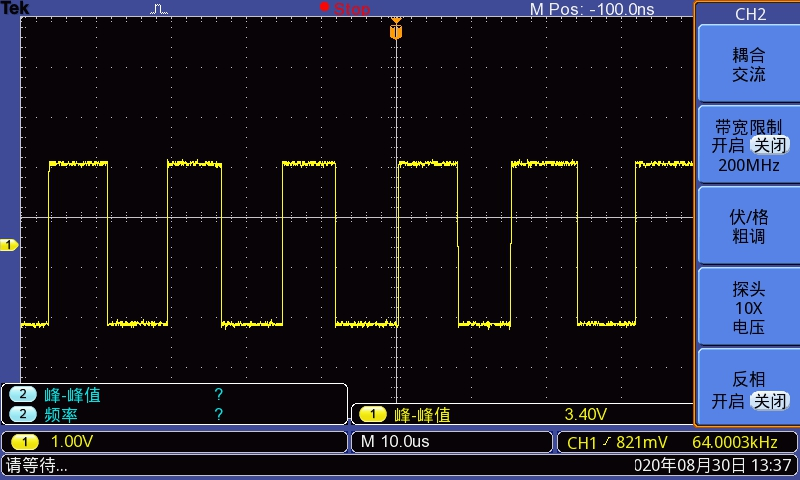
\includegraphics[
      width = \linewidth,
    ]{phase}
    \caption{相频特性}%
    \label{fig:phase}
  \end{subfigure}
  \caption{特性曲线}%
  \label{fig:character}
\end{figure}

\subsubsection{分别利用上述两个滤波器对被抽样信号进行恢复,比较被抽样信号恢复效果}%
\label{ssub:recover}

% \begin{table}[htbp]
%   \centering
%   \caption{连线}%
%   \label{tab:\arabic{chapter}\arabic{subsection}recover}
%   \small
%   \csvautobooktabular[respect percent]{tab/\arabic{chapter}\arabic{subsection}recover.csv}
% \end{table}

% \begin{enumerate}
%   \item 关电,按表格所示进行连线:
%   \item 开电,设置主控菜单,选择【主菜单】→【通信原理】→【抽样定理】→【FIR 滤
%     波器】。调节 W1 (主控\& 信号源) 使信号 A-OUT 输出峰峰值为 3V 左右。
%   \item 此时实验系统初始状态为:待抽样信号 MUSIC 为 3K+1K 正弦合成波,抽样时
%     钟信号 A-OUT 为频率 9kHz、占空比 20\%的方波。
%   \item 实验操作及波形观测。


对比观测不同滤波器的信号恢复效果:用示波器分别观测 LPF-OUT3\# 和译码输出 3\#
,以 100Hz 步进减小抽样时钟 A-OUT 的输出频率,对比观测模拟滤波器
图~\ref{fig:compare/analog}和 FIR 数字滤波器图~\ref{fig:compare/fir}在不同
抽样频率下信号恢复的效果。(频率步进可以根据实验需求自行设置。)

\begin{figure}[htbp]
  \centering
  \begin{subfigure}[htbp]{0.45\linewidth}
    \centering
    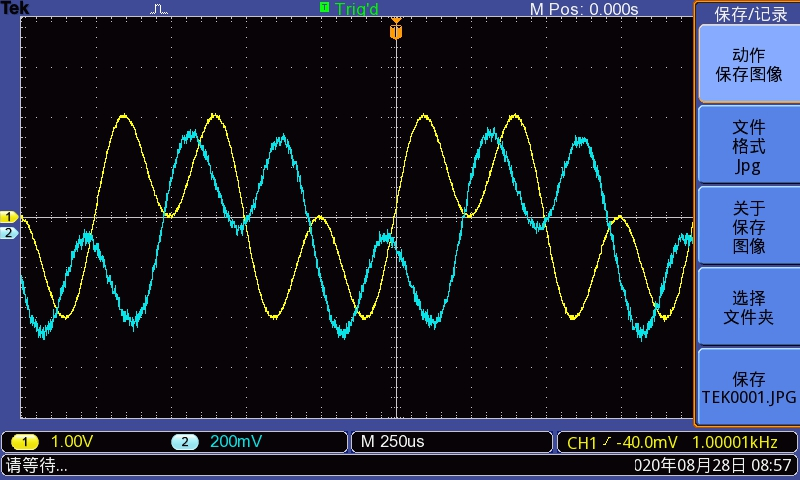
\includegraphics[
      width = \linewidth,
    ]{compare/analog}
    \caption{模拟低通滤波未失真}%
    \label{fig:compare/analog}
  \end{subfigure}
  \quad
  \begin{subfigure}[htbp]{0.45\linewidth}
    \centering
    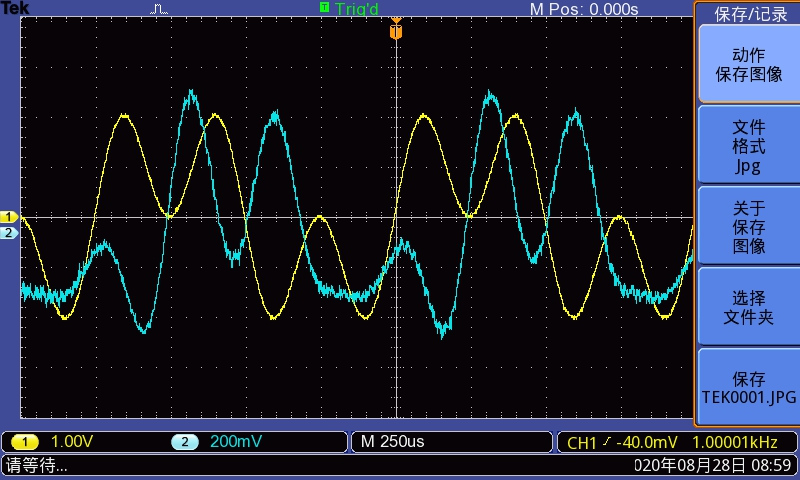
\includegraphics[
      width = \linewidth,
    ]{compare/fir}
    \caption{FIR 已经失真}%
    \label{fig:compare/fir}
  \end{subfigure}
  \caption{对比}%
  \label{fig:compare}
\end{figure}

% \end{enumerate}

\begin{Exercise}[title = 思考, label = ex:filter]
  不同滤波器的幅频特性对抽样恢复有何影响?
\end{Exercise}

\begin{Answer}
  抽样恢复信号频谱是抽样输出信号频谱与滤波器的频谱特性乘积。

  当抽样信号未发生混叠的时候,可以通过截止频率为最高频率2倍的理想带通滤波器来
  恢复原信号。

  但因为所有滤波器都不是由理想低通滤波器,所以都会有一定程度的失真。在本实验
  中,如图~\ref{fig:compare}所示,截至频率 3kHz 的 FIR 滤波器不如 3.4kHz 的模
  拟低通滤波器,原因是模拟低通滤波器的截至频率是 3.4kHz,而 FIR 滤波器是在
  3kHz,而信号最高频率是 3kHz, FIR 滤波器没有预留余量,会有一定失真。
\end{Answer}

\subsection{滤波器相频特性对抽样信号恢复的影响}%
\label{sub:phase}

% 该项目是通过改变不同抽样时钟频率,从时域和频域两方面分别观测抽样信号经 fir 滤
% 波和 iir 滤波后的恢复失真情况,从而了解和探讨不同滤波器相频特性对抽样信号恢复
% 的影响。

\subsubsection{观察被抽样信号经过 fir 低通滤波器与 iir 低通滤波器后,所恢复信号的频谱}%
\label{ssub:freq}

% \begin{table}[htbp]
%   \centering
%   \caption{连线}%
%   \label{tab:\arabic{chapter}\arabic{subsection}freq}
%   \small
%   \csvautobooktabular[respect percent]{tab/\arabic{chapter}\arabic{subsection}freq.csv}
% \end{table}

% \begin{enumerate}
%   \item 关电,按表~\ref{tab:\arabic{chapter}\arabic{subsection}freq}所示进行
%     连线。
%   \item 开电,设置主控菜单,选择【主菜单】→【通信原理】→【抽样定理】。调节 W1
%     (主控\&信号源) 使信号 A-OUT 输出峰峰值为 3V 左右。
%   \item 此时实验系统初始状态为:待抽样信号 MUSIC 为 3K+1K 正弦合成波,抽样时
%     钟信号 A-OUT 为频率 9kHz、占空比 20\%的方波。
%   \item 实验操作及波形观测。
  \begin{enumerate}
    \item 观测信号经 fir 滤波后波形恢复效果:设置主控模块菜单,选择【抽样定理
      】→【FIR 滤波器】;设置【信号源】使 A-OUT 输出的抽样时钟频率为 7.5kHz;
      用示波器观测恢复信号译码输出 3\#的波形图~\ref{fig:recover/fir_wave}和频
      谱图~\ref{fig:recover/fir_spectrum}。
    \item 观测信号经 iir 滤波后波形恢复效果:设置主控模块菜单,选择【抽样定理
      】→【IIR 滤波器】;设置【信号源】使 A-OUT 输出的抽样时钟频率为 7.5kHz;
      用示波器观测恢复信号译码输出 3\#的波形图~\ref{fig:recover/iir_wave}和频
      谱图~\ref{fig:recover/iir_spectrum}。
    \item 探讨被抽样信号经不同滤波器恢复的频谱和时域波形:

      \begin{Exercise}[title = 思考]
        被抽样信号与经过滤波器后恢复的信号之间的频谱是否一致?如果一致,是否
        就是说原始信号能够不失真的恢复出来?用示波器分别观测 fir 滤波恢复
        图~\ref{fig:recover/fir_wave}和 iir 滤波恢复情况
        图~\ref{fig:recover/iir_wave}下,译码输出3\# 的时域波形是否完全一致,
        如果波形不一致,是失真呢?还是有相位的平移呢?如果相位有平移,观测并
        计算相位移动时间。
      \end{Exercise}

      \begin{Answer}
        被抽样信号与经过滤波器后恢复的信号之间的频谱不一致。原始信号不能够不
        失真的恢复出来,因为滤波器的频谱特性不够理想,也不是理想的线性相频特
        性。fir 和 iir 都有一定的失真。有 0.25 ms 的相位平移。
      \end{Answer}
  \end{enumerate}
% \end{enumerate}

\begin{figure}[htbp]
  \centering
  \begin{subfigure}[htbp]{0.45\linewidth}
    \centering
    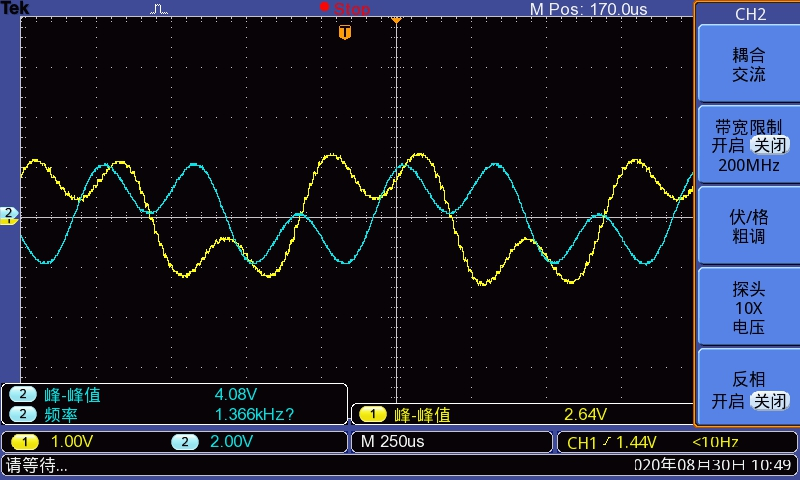
\includegraphics[
      width = \linewidth,
    ]{recover/fir_wave}
    \caption{fir 波形}%
    \label{fig:recover/fir_wave}
  \end{subfigure}
  \quad
  \begin{subfigure}[htbp]{0.45\linewidth}
    \centering
    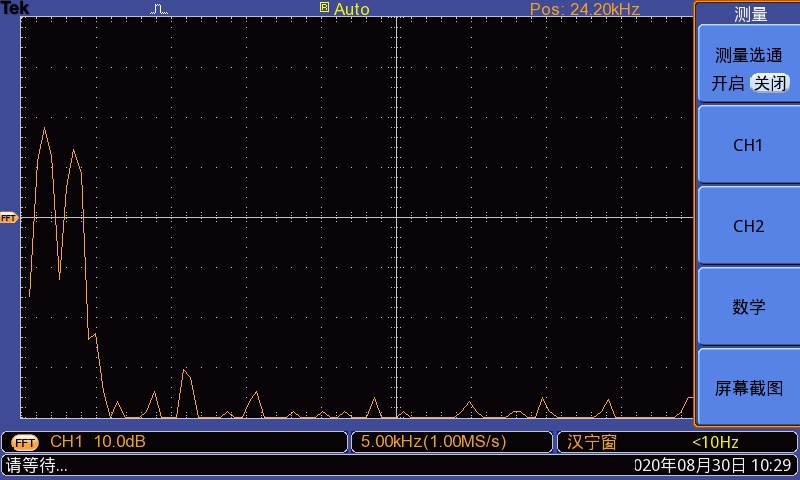
\includegraphics[
      width = \linewidth,
    ]{recover/fir_spectrum}
    \caption{fir 频谱}%
    \label{fig:recover/fir_spectrum}
  \end{subfigure}

  \begin{subfigure}[htbp]{0.45\linewidth}
    \centering
    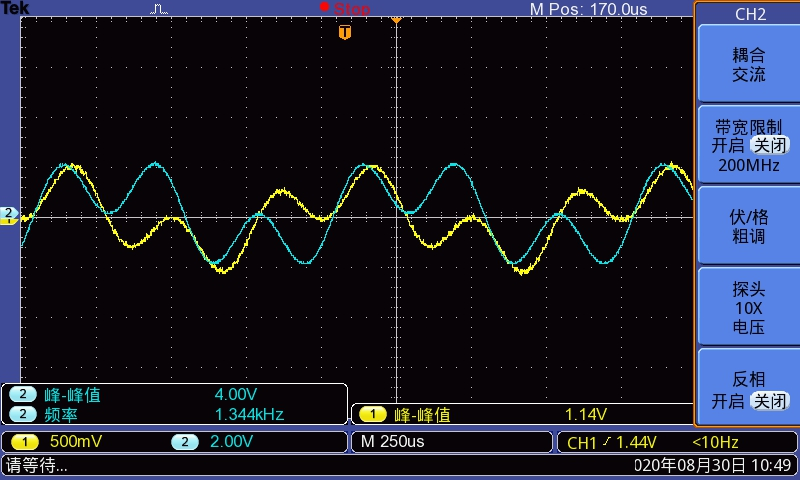
\includegraphics[
      width = \linewidth,
    ]{recover/iir_wave}
    \caption{iir 波形}%
    \label{fig:recover/iir_wave}
  \end{subfigure}
  \quad
  \begin{subfigure}[htbp]{0.45\linewidth}
    \centering
    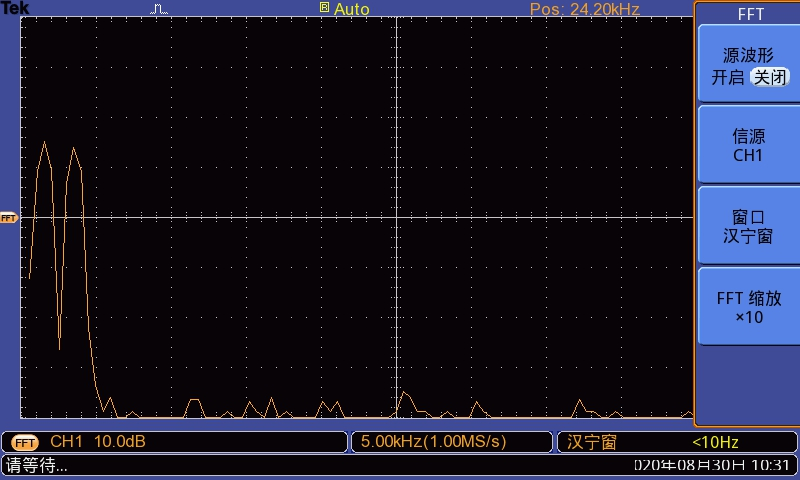
\includegraphics[
      width = \linewidth,
    ]{recover/iir_spectrum}
    \caption{iir 频谱}%
    \label{fig:recover/iir_spectrum}
  \end{subfigure}
  \quad
  \caption{还原}%
  \label{fig:recover}
\end{figure}

% 注:实际系统中,失真的现象不一定是错误的,实际系统中有这样的应用。

\subsubsection{观测相频特性}%
\label{ssub:phase}

% \begin{table}[htbp]
%   \centering
%   \caption{连线}%
%   \label{tab:\arabic{chapter}\arabic{subsection}phase}
%   \csvautobooktabular[respect percent]{tab/\arabic{chapter}\arabic{subsection}phase.csv}
% \end{table}

% \begin{enumerate}
%   \item 关电,按表~\ref{tab:\arabic{chapter}\arabic{subsection}phase}所示进行连线。
%   \item 开电,设置主控菜单,选择【主菜单】→【通信原理】→【抽样定理】→【FIR 滤波器】。
%   \item 此时系统初始实验状态为: A-OUT 为频率 9kHz、占空比 20\%的方波。
%   \item 实验操作及波形观测。

    对比观测信号经 fir 滤波后的相频特性:设置【信号源】使 A-OUT 输出频率为
    5kHz、峰峰值为 3V 的正弦波;以 100Hz 步进减小 A-OUT 输出频率,用示波器对
    比观测 A-OUT (主控\&信号源)和译码输出3\# 的时域波形
    图~\ref{fig:recover/fir_wave}。相频特性测量就是改变信号的频率,测输出信号
    的延时(时域上观测)。记入表和图~\ref{fig:phase}。
% \end{enumerate}

% \begin{table}[htbp]
%   \centering
%   \caption{相频特性}%
%   \label{tab:phase}
%   \tiny
%   \csvautobooktabular[respect percent]{tab/phase.csv}
% \end{table}

\section{实验报告}%
\label{sec:\arabic{chapter}report}

\begin{Exercise}
  分析电路的工作原理,叙述其工作过程。
\end{Exercise}

\begin{Answer}
  工作原理见图~\ref{fig:\arabic{chapter}dia},工作过程见
  章节~\ref{sec:\arabic{chapter}principle}。
\end{Answer}

\begin{Exercise}
  绘出所做实验的电路、仪表连接调测图。并列出所测各点的波形、频率、电压等有关
  数据,对所测数据做简要分析说明。必要时借助于计算公式及推导。
\end{Exercise}

\begin{Answer}
  实验的电路、仪表连接调测图见图~\ref{fig:\arabic{chapter}dia},被抽样信号波
  形、电压见图~\ref{fig:sample/flat}和频率、电压见
  图~\ref{fig:freqsample/unsample},平顶抽样信号波形、电压见
  图~\ref{fig:sample/flat},自然抽样信号波形、电压见
  图~\ref{fig:sample/nature}和频率、电压见图~\ref{fig:freqsample/sample},模
  拟低通滤波输出频率、电压见图~\ref{fig:freqsample/lp}, fir 低通滤波输出波形
  、电压见图~\ref{fig:recover/fir_wave}和频率、波形见
  图~\ref{fig:recover/fir_spectrum}, iir 低通滤波输出波形、电压见
  图~\ref{fig:recover/iir_wave}和频率、波形见
  图~\ref{fig:recover/iir_spectrum}。

  分析:音乐信号$x(t)$经过$\sum^\infty_{n = -\infty} \delta(t -
  nT_\mathrm{s})$自然采样后$x_\mathrm{s}(t)$出现了周期延拓,经过
  $\mathrm{rect}(\frac{f}{f_\mathrm{s}})$低通滤波后选通了其中一个周期,从而还
  原了信号。
\end{Answer}

\begin{align}
  x(t) * \sum^\infty_{n = -\infty} \delta(t - nT_\mathrm{s}) = & x_\mathrm{s}(t)\\
  X(f) \sum^\infty_{n = -\infty} \delta(f - nf_\mathrm{s}) = & X_\mathrm{s}(f)\\
  X_\mathrm{s}(f) \mathrm{rect}(\frac{f}{f_\mathrm{s}}) = & X(f)
\end{align}

\begin{Exercise}
  分析以下问题:滤波器的幅频特性是如何影响抽样恢复信号的?简述平顶抽样和自然
  抽样的原理及实现方法。
\end{Exercise}

\begin{Answer}
  分析见问题~\ref{ex:filter}(这2个问题重复了)。
\end{Answer}

\begin{description}
  \item[平顶抽样]具有一定持续时间,在持续时间内幅度不变。等效为通过一个线型网
    络$H(f)$,实现:通过脉冲抽样后经过一保持器;
  \item[自然抽样]理想的自然抽样是一个持续时间为0的信号,但实际矩形的脉冲抽样
    会导致出现 sinc 函数的延拓。实现:直接与抽样脉冲相乘。
\end{description}

\begin{Exercise}
  思考一下,实验步骤中采用 3K+1K 正弦合成波作为被抽样信号,而不是单一频率的正
  弦波,在实验过程中波形变化的观测上有什么区别?对抽样定理理论和实际的研究有
  什么意义?
\end{Exercise}

\begin{Answer}
  区别是正弦合成波更加稳定,更容易观测到频谱混叠现象。而且2条谱线比多条谱线视
  觉上更加清楚,便于分析。

  意义是实际的被抽样信号一般都是多频而非单一频谱的,所以更贴近实际。
\end{Answer}

\end{document}
